\chapter{Guy - \emph{Interface Graphique}}

Nous avons fait l'interface graphique en HTML/CSS et Javascript. Le fait d'avoir
l'interface graphique sur le web nous permet de le deployer sur internet et de
permettre à quiconque de lancer notre programme depuis n'importe où.

\section{Scénario}

Le scénario est très simple. En quelques clics, l'utilisateur peut utiliser
notre programme.

\begin{enumerate}
  \item L'utilisateur se rend sur le site dans la partie "Run Online" dédiée à
    l'utilisation de notre programme d'OCR à distance.
  \item L'utilisateur choisi son image (sur son ordinateur, en local) et
    l'upload sur le serveur. (Des tests sont bien évidemment effectués sur le
    fichier envoyé par l'utilisateur, parmi lesquels un test sur la taille du
    fichier (pour limiter le risque d'un espace disque plein), des tests sur le
    MIME type du fichier - pour s'assurer que c'est bien une image)

    \begin{center}
      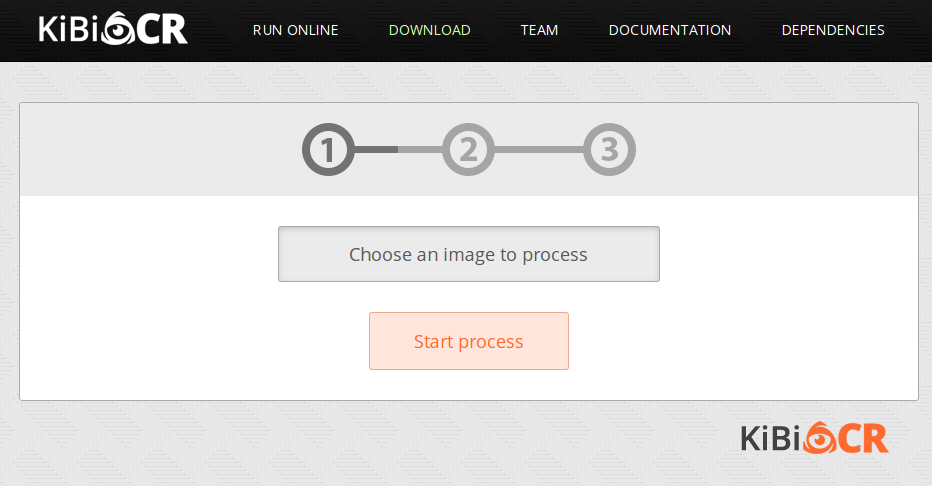
\includegraphics[scale=0.35]{chapters/Pictures/toogy/guy.png}
    \end{center}

  \item Le démon qui attend qu'une nouvelle image soit uploadée reçoit
    l'information de l'upload. Il s'occupe de simplement faire appel au
    programme kibiocr installé sur le système. Le démon communique en temps réel
    des informations sur les étapes en cours du programme et le temps qu'elle
    prennent à l'utilisateur afin que celui-ci ne s'impatiente pas. Ces données
    sont reçues par le navigateur, via javascript, et affichée dans le HTML.
    
    \begin{center}
      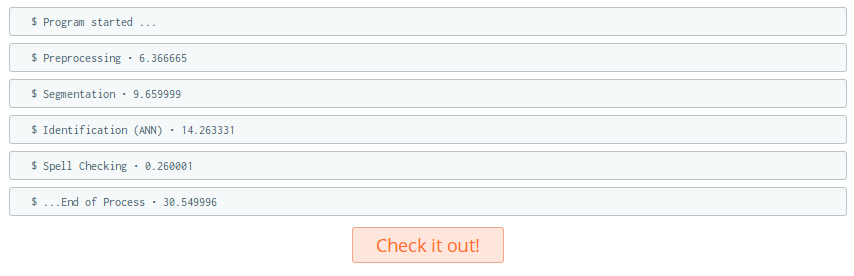
\includegraphics[scale=0.42]{chapters/Pictures/toogy/guy-process.png}
    \end{center}
  \item Une fois le process fini, le résultat de l'identification des caractères
    ainsi que l'analyse syntaxique de la langue (propositions de corrections)
    sont envoyés au programme javascript qui va alors l'afficher à l'utilisateur
    une fois que celui-ci aura cliqué sur le bouton qui lui permet d'afficher le
    résultat du programme appliqué à l'image de son choix.
    
    \begin{center}
      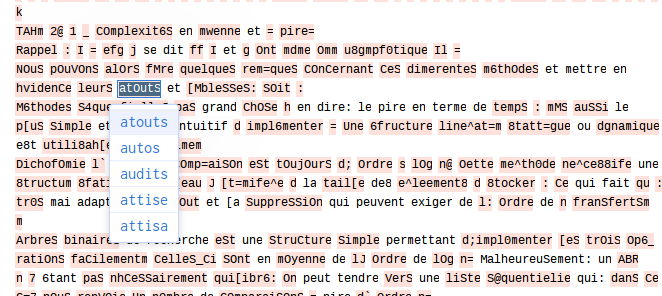
\includegraphics[scale=0.55]{chapters/Pictures/toogy/guy-robert.png}
    \end{center}
\end{enumerate}

\begin{figure}[h!]
  \centering
  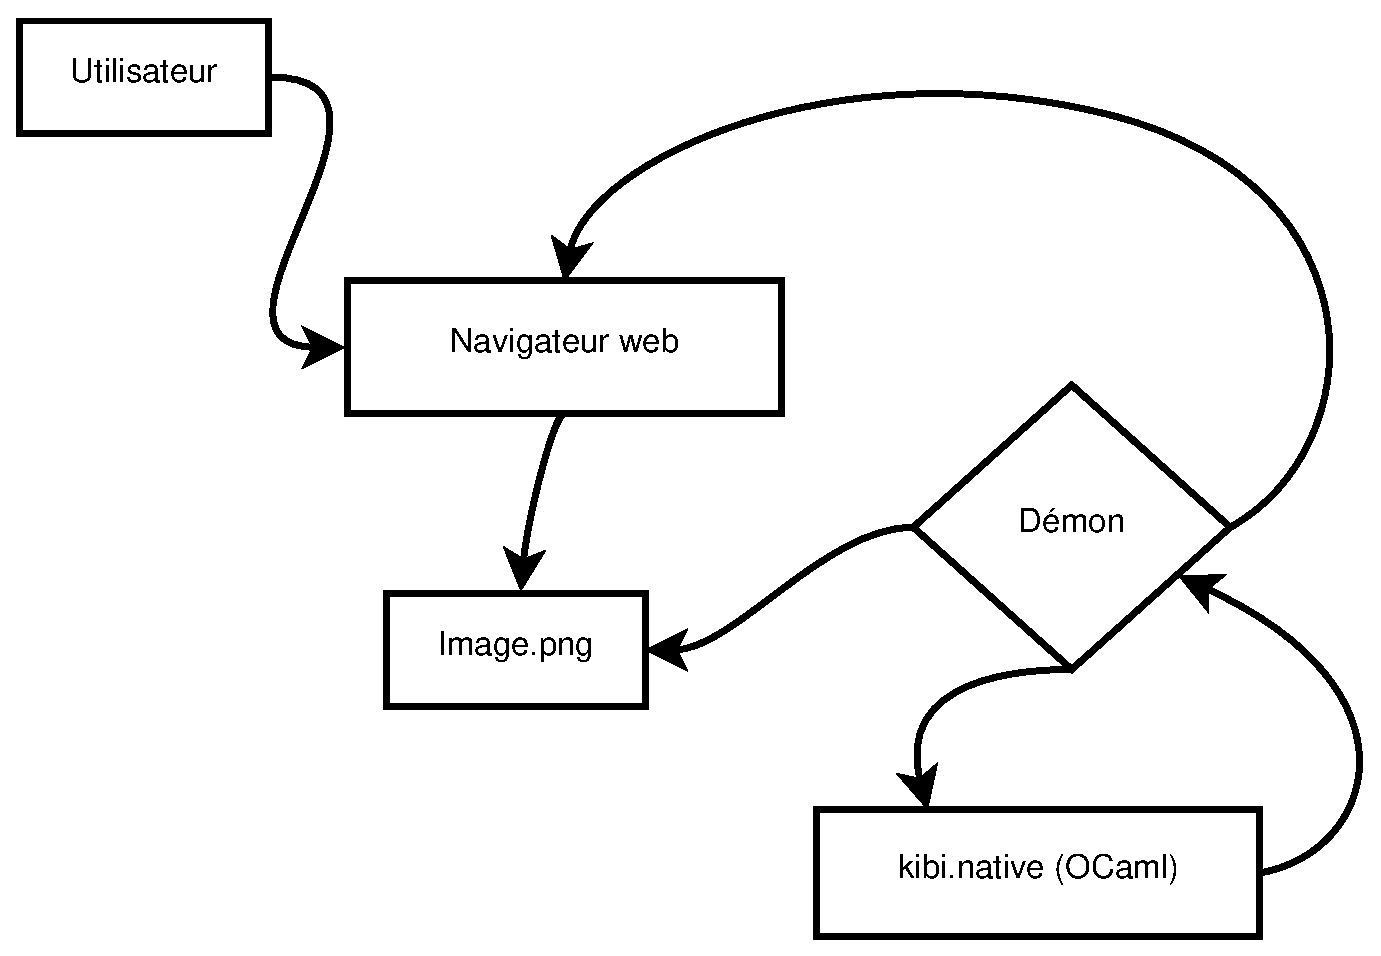
\includegraphics[scale=0.4]{chapters/Pictures/toogy/guy-scenario.eps}
  \caption{Schéma récapitulant le scénario d'utilisation du programme}
\end{figure}

\section{Serveur web}

Qui dit interface web dit serveur web. Le serveur web que nous utilisons est
nginx. Il est facile à installer et à configurer.

